% !TeX program = pdfLaTeX
% \documentclass[smallextended]{svjour3}       % onecolumn (second format)
\documentclass[twocolumn]{svjour3}          % twocolumn
%
\smartqed  % flush right qed marks, e.g. at end of proof
%
\usepackage{amsmath}
\usepackage{graphicx}
\usepackage[utf8]{inputenc}
\usepackage{eurosym}
\usepackage{svg}
\usepackage{eurosym}
\usepackage[hyphens]{url} % not crucial - just used below for the URL
\usepackage{hyperref}
\providecommand{\tightlist}{%
  \setlength{\itemsep}{0pt}\setlength{\parskip}{0pt}}

%
% \usepackage{mathptmx}      % use Times fonts if available on your TeX system
%
% insert here the call for the packages your document requires
%\usepackage{latexsym}
% etc.
%
% please place your own definitions here and don't use \def but
% \newcommand{}{}
%
% Insert the name of "your journal" with
% \journalname{myjournal}
%

%% load any required packages here

\PassOptionsToPackage{language=auto,backref=true,urldate=iso,seconds=true,date=iso, datamodel=custom,datecirca=true, dateuncertain=true}{biblatex}
\usepackage{biblatex}
   \addbibresource{mybibfile.bib}

\usepackage[abbreviations]{foreign}
\usepackage{bbm}
% \usepackage{cleveref}
\usepackage{amsmath}
% \usepackage{glossaries-extra}
\usepackage{paralist}
\usepackage{glossaries}
\usepackage{tabularx}
\usepackage{csquotes}
\usepackage{booktabs}
\usepackage{hyperref}
\usepackage[utf8]{inputenc}
\usepackage[hyperref,framed]{ntheorem}
\newtheorem{hypo}{Hypothesis}
\PassOptionsToPackage{pdftex,hyperfootnotes=false,pdfpagelabels,bookmarksdepth=3}{hyperref}
\usepackage[all]{hypcap}
\usepackage{hyphenat}
\hypersetup{ colorlinks=false, linktocpage=true}
\usepackage{caption}

\makeglossaries

\begin{document}

\newacronym{loa}{LoA}{Level of Automation}
\newacronym{sar}{SAR}{Socially Assistive Robot}
\newacronym{ldb}{LdB}{Learning by Demonstration}
\newacronym{hci}{HCI}{Human-Computer Interaction}
\newacronym{hra}{HRA}{Human-Robot Alliance}
\newacronym{hri}{HRI}{Human-Robot Interaction}
\newacronym{mab}{MAB}{Multi-Armed Bandit Problem}
\newacronym{dts}{DTS}{Double Thompson Sampling}
\newacronym{rmed}{RMED}{}
\newacronym{wai}{WAI}{Working Alliance Inventory}
\newacronym{rosas}{RoSAS}{Robot Social Attribute Scale}
\newacronym{nars}{NARS}{Negative Attitudes Towards Robots}
\newacronym{sus}{SUS}{System Usability Scale}
\newacronym{paes}{PAES}{Physical Enjoyment Scale}
\newacronym{woz}{WoZ}{Wizard of Oz}




% \newglossaryentry{adt}{name=ADT, description={Atlantic Daylight Time}}
% \newglossaryentry{est}{name=EST, description={Eastern Standard Time}}


\title{Out-of-the-Box? Using Preference Learning to Personalize Human-Robot Interaction}
\subtitle{Adaptive Robot Exercising Companions are Perceived as More Competent and Trustworthy}



\author{ Sebastian Schneider \and Franz Kummert }


\institute{
    }

\date{Received: date / Accepted: date}
% The correct dates will be entered by the editor


\maketitle


\begin{abstract}

Learning and matching a user's preference is an essential aspect of
achieving a productive collaboration in long-term \gls{hri}. However, there are different techniques on how to match the
behavior of a robot to a user's preference. The robot can be \textit{adaptable}
so that a user can change the robot's behavior to one's need, or the
robot can be \textit{adaptive} and autonomously tries to match its behavior
to the user's preference. Both types might decrease the gap between a user's preference and the actual system behavior. However, the \gls{loa} of
the robot is different between both methods. Either the user controls
the interaction, or the robot is in control. In this paper, we present a
study on the effects of these different \gls{loa} of a \gls{sar} on a user's evaluation of the system in an exercising
scenario. We implemented an online preference learning system and a user-adaptable system. We conducted a between-subject design study (\textit{adaptable} robot
vs.~\textit{adaptive} robot) with 40 subjects. The results show that users
evaluate the \textit{adaptive} robots as more competent, warm and report a higher
alliance. Moreover, this increased alliance is significantly mediated by
the perceived competence of the system. This result provides empirical
evidence for the relation between the \gls{loa} of a system, the user's
perceived competence of the system and the perceived alliance with it.
\\
\keywords{ Human-Robot Interaction, Preference Learning, Adaptive Robots, User Experience
    }


\end{abstract}


\def\spacingset#1{\renewcommand{\baselinestretch}%
{#1}\small\normalsize} \spacingset{1}


\hypertarget{introduction}{%
\section{Introduction}\label{introduction}}

Future scenarios of social robots envision a personalizable system that is flexible and adapts itself to the user's preferences~\autocite{leite}. 
However, building a customized system for each user is not feasibile. Thus, anticipating every potential user type and pre-programing the system for their needs will be an obstacle to deploy robots in domestic settings that engage the users beyond a technologz exploration phase. Thus, robots should have capabilities to adjust to different users profiles (\eg{}, match a user's personality \autocite{andrist2015look}). Adapting to different users and therefore enhancing the interaction experience is widely implemented in web-based applications (e.g., recommender systems on Amazon, Google, eBay, Netflix). 
However, adaptation remains a challenging issue for social robots that are not attached to a large user database which could enable techniques like collaborative filtering. 
Therefore, social robots are likely to face the so called \textit{cold start problem}, which requires the system to gather initial user data to personalize the interaction experience. Hence, deploying an \textit{adaptive} system comes with some known difficulties:

First, querying the user for information in real time \gls{hri} might be more
cost-intensive than in web-based applications.~\textcite{cakmak2010designing} showed that a constant stream of questions in a~\gls{ldb} task annoys users.

Second, robots making autonomous personalization
decisions could result in diametral effects for the user's ~\gls{hri} experience satisfaction. Having the robot in control of the interaction personalization could lead to a disuses of the technology. This is plausible either when the systems learns a wrong user profile or when the user preferes to be in control of the interaction~\cite{burger2013desire}. Thus, it is essential to consider whether it is also sufficient to just provide an interface for the human to adjust the system's behavior instead of having the robot adapt by itself.
These different types of possible personalization strategies would influence the autonomy of the system, which in turn might affect the interaction experience in different ways.
Based on~\citeauthor{epley2007seeing}'s theory of anthropomorphization, an autonomous \textit{adaptive} system could create an unexpected experience for the user~\autocite{epley2007seeing}. This unexpected experience could increase a user's perceived anthropomorphization of the robot. Furthermore, this higher degree could enhance the credibility of the system and might influence the trust in it. In contrast, a system that is controlled and adjusted by the user should increase the match between the robot's behavior and the user's expectation and therefore reduce anthropomorphic effects. The investigation of these two aspects is the core of this work. We try to find an answer to the question:

What effects have different types of a robot's personlization methods on the
user's perception of the system, trust in the alliance and motivation to interact with the
system?

To investigate the effects of different preference matching behaviors of
the system, this work presents a study in the area of robotic exercising companiosn that compares the impact of having
an~\textit{adaptive} robot versus an~\textit{adaptable} robot as an exercising partner for
physical activities. This work is therefore a continuation of previous endeavours of building socially assistive robot exercising companions. Previous work on robots for exercising and coaching have investigated the motivational effects of using such coaching systems~\autocite{fasola2013socially,schneider2016exercising,guneysu2017}.
However, most of the previous studies used only one type of exercises (\eg{}, arm or plank exercises). Thus, the users could not choose between different exercises. In this work, we present a system that offers a range of exercises to the user and raises the question of what
is a suitable preference matching framework to provide a personalized preference-based interaction. Therefore, in the~\textit{adaptive} condition, the robot proposes different activities for the user and tries to learn an exercising preference ranking of the user based on comparative user preference feedback. In the~\textit{adaptable} condition, the robot is directly controlled by the user, and the user can decide what kind of exercises they want to do together with the robot.

\subsection{Objectives and Contribution}
To summarize, this paper has two major objectives. The first objective is to test whether a preference learning approach\footnote{(\ie{}, k-armed Dueling Bandit Learning)} is suitable for online interaction which is novel for the~\gls{hri}community and test the feasibility in a realistic use case study in comparison to a user-controlled adjustment method. 

The second objective is to investigate how the different personalization methods influence the user's evaluation of the system in terms of its social attributes, trust in the alliance with the system and the motivation to continue the interaction with it. 

Our work contributes to the community by showing that k-armed Dueling Bandit Problem is a suitable approach for online preference learning in~\gls{hri} scenarios. Moreover, we provide evidence that the alliance to an adaptive robotic exercising partner is perceived as more trustworthy and that this is mediated by a perceived higher competence of the system by the user.


\subsection{Organization}

The difference between \textit{adaptive} and \textit{adaptable} robots will be explained
in \autoref{adaptation:sec:background} along with the concepts of
automation and alliance, which might be important variables when
looking at the adaptivity of a system. Section \ref{adaptation:sec:system}
introduces the system design and \autoref{adaptation:sec:study} explains the
study design to test the effects of a robot's different personalization
mechanisms. Section \ref{adaptation:sec:results} presents the results of the
study, which are discussed in \autoref{discussion}. Finally,
~\autoref{adaptation:sec:conclusion} gives a conclusion of this work.

\hypertarget{adaptation-automation-and-alliance}{%
\section{\texorpdfstring{Adaptation, Automation and Alliance
\label{adaptation:sec:background}}{Adaptation, Automation and Alliance }}\label{adaptation-automation-and-alliance}}

This section gives a brief introduction into the concepts of adaptation,
automation and alliance. Discussing these topics is a challenging task
because they are used differently across disciplines (\eg{}, philosophy,
psychology, economics, biology). Therefore, the following explanations
can not be exhaustive and will focus mainly on a computer science and
psychology perspective.

\hypertarget{adaptation-adaptivity-versus-adaptability}{%
\subsection{Adaptation: adaptivity versus
adaptability}\label{adaptation-adaptivity-versus-adaptability}}

In computer science adaptation referes to the informative-based process of adjusting the behavior of an interactive system to meet the need of individual users \cite{schneider1993adaptive}.
Even though computer software or robots are running through many
software design cycles, it is hard to anticipate the requirements for
every possible user. The goal of the \textit{adaptive} process is to minimize the
discrepancy between the user needs and system behavior after the
deployment. This \textit{adaptive} process can either be automatically initiated
by the system, in this case, the system is \textit{adaptive} (\eg{}, the system
chooses exercises for the users by itself), or us Sie können Felix Busch gerne meinen Lebenslauf schicken. Benötigen Sie eine deutsche Version oder reicht eine englische?ers can adjust the
system by themselves, in this case the system is \textit{adaptable} (\eg{}, the
users can choose the exercises by themselves). Adaptation can be based
on different user profiles (\eg{}, age, gender, personality), various
times (\eg{}, morning/evening, days of the week, summer/winter) or other
user characteristics (\eg{}, mood, expertise over time).

\begin{figure}[h!]
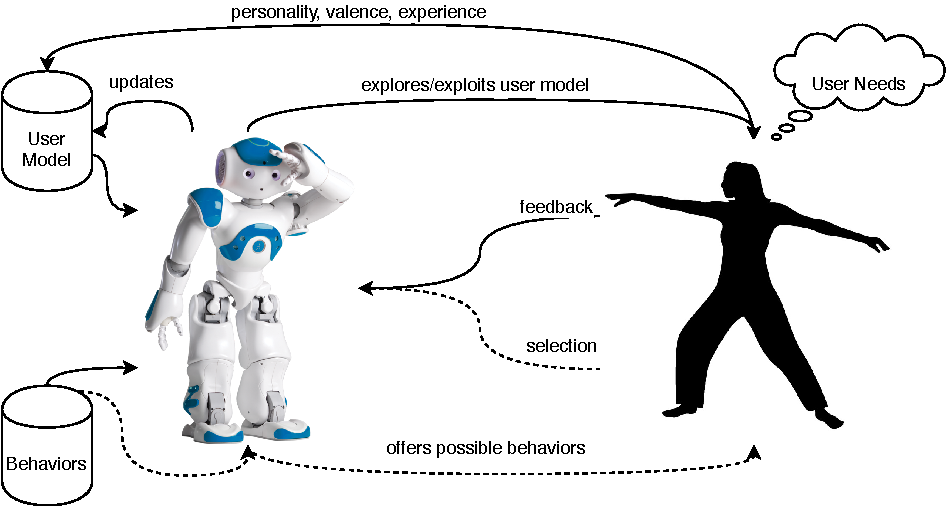
\includegraphics[width=\columnwidth]{figures/figure-latex/adaptation.pdf}
\caption{The adaptable system (dashed lines) comes with a set of behaviors it can offer to the user. The user selects her/his preferred behavior and the system performs the action. The adaptive system (solid lines) explores which behavior is preferred by the user by querying prefernce feedback. The system updates it's user model and can exploit the obtained information over time. Alternatively, the system can also make stereotypical predictions based on the user personality, as well as the valence or exerperience of the user. } \label{fig:adaptation}
\end{figure}

Previous work in \gls{hri}investigated the implementation of \textit{adaptive}
processes to match a user's personality, generate empathic behavior,
adapt therapy sessions, interaction distance, linguistic style or puzzle skills.
\autocites{tapus2008user,leite2011modelling,Tsiakas2016,mitsunaga2008adapting,ritschel,leyzberg2014personalizing,hemminghaus2017towards}.
The results of these works show show an improvement in task performance based on personalized lessons or user personality matching \cite{tapus2008user, leyzberg2014personalizing,hemminghaus2017towards}. Additionally, providing adaptive empathic feedback also improved user engagement \cite{leite2011modelling}. Other works present evidence for the feasability of certain adaptation algorithms (\eg{}, \cite{mitsunaga2008adapting}). Overall, there is evidence that adaptive personalization is a crucial capability for robots. Though, there are still many open issues that future works need to target. For example, what are the best objectives for the robot to adapt to? How can the system adapt when the objective are not evident? Should the adaptation process be communicated and transparent and who should be in control of the adaptation process?

Although some have compared \textit{adaptive} robots with experimental baseline
control conditions (\eg{}, \autocite{leite2011modelling,leyzberg2014personalizing}), to the
best of our knowledge, no investigation looked at the effects of robot-initiated
personalization versus user-initiated personalization. It is reasonable
to argue that the users could control and adjust the robot behavior to
their preferences. Leyzberg et al.~\autocite{leyzberg2014personalizing},
for example, investigated the effects of a robot that gives personalized
lessons to the user. These tutorials are selected by the robot's
decisions. However, also the user could have requested for a specific
lesson.

Both strategies might match a user's preference and increase the
interaction satisfaction, but the underlying difference in decision
making is fundamental. One can interpret the different strategies as
either more transparent or as more competent. Generally, the question of
whether to build an \textit{adaptive} or \textit{adaptable} system raises the concern of
who is in control and how does it affect the interaction experience. The
issue of who is in control is, in general, associated with the \gls{loa} of the system.

\hypertarget{level-of-automation}{%
\subsection{Level of Automation}\label{level-of-automation}}

An autonomous agent acts based on the information it receives from its
sensors, knows in which state it is and makes a decision accordingly
which is associated with an agent's action
\autocite[see][ch.~1]{russell2016artificial}. \gls{loa} of a system changes an
agent's capability to act and react based on information on its own
without any other external control instances. Thus, the \gls{loa} of an agent
is altered by the task and environment of the agent and whether a human
can interfere with an agent's control loop.

It becomes essential were robots are carrying out delicate tasks (\eg{},
lethal autonomous weapons). There are various frameworks that can be
used to identifiy the \gls{loa} of a system
(\eg{},\autocite{sheridan1978human,endsley1995out}). However, most
recently, \textcite{beer2014toward} have proposed a taxonomy to classify
the level of robot autonomy for~\gls{hri}.

Regardless of the exact different \gls{loa}, systems can be categorized as
human-in-the-loop systems where the human has to approve a control
decision by the autonomous agents, human-on-the-loop where the human is
informed about decision but the agent would carry out a decision if the
human operator is not interfering or human-off-the-loop, where a human
cannot interfere with the agent's
decisions\footnote{Earliest examples of hands-off-the-loop agents are land and naval mines.}.

The relevance to consider different \gls{loa} are apparent in sensible domains
such as military operations or medical applications (\eg{}, surgery or
medicine dispenser), but (yet) less apparent in socially assistive
domains (\eg{}, rehabilitation or teaching). Nevertheless, also social
situations will require to understand whether a social robot should act
autonomously, semi-self controlled or is in full human control. For the
interaction experience it will be crucial to understand the effects of
different \gls{loa}. In the course of this work, we are interested in the
effects of whether a robot exercising companion is in control to choose
the exercises or the users can decide which exercises they want to do.
The question of whether the \gls{loa} is appropriate and which effects it will
have on the interaction will be related to the alliance and trust
between the users and the \gls{sar}.
\autocite{beer2014toward}.

\hypertarget{alliance-and-trust}{%
\subsection{Alliance}\label{alliance-and-trust}}

The impact of trust in alliance between a user and a robot has recently been investigated in use cases in which a
robot shows a faulty behavior, gives explanations for actions, or varies
the degree of expressivity and vulnerability
\autocite{salem2015would,robinette2016overtrust,Wang,Martelaro} Besides
these aspects, it is significantly related to whether humans trust a
robot's capabilities if the systems has, for example, a high \gls{loa} and makes autonomous decisions.
\autocite{freedy2007measurement}.

Trust is defined in \gls{hci} as \enquote{the extent
to which a user is confident in and willing to act by, the
recommendations, actions, and decisions of an artificially intelligent
decision aid} \autocite[p.~25]{mcallister1995affect}. As Madsen et
al.~\autocite{madsen2000measuring} state, this definition
\enquote{encompasses both the user's confidence in the system and their
willingness to act on the system's decision and advice}
\autocite[p.~1]{madsen2000measuring}. Thus, it already incorporates a
notion of user trust regarding the willingness to take a system's
recommendations into account.

To understand how trust influences \gls{hri},~\textcite{hancock2011meta} reviewed different applications where
confidence is an essential factor when robots and humans are working
together in a team. They state that it is a crucial aspect of industry,
space or warfare applications. Additionally, trust will also be
essential to understanding social tasks due to the rise of \gls{sar} for
rehabilitative, therapeutic or educational tasks
\autocite{corry,fasola2013socially}.~\citeauthor{hancock2011meta} found several
factors influencing trust in \gls{hri}, which are related to the human, the
robot, and the environment. However, the robot related factors were the
most important ones in their meta-review. They found that essential
factors influencing the associated trust are the human's perception of
the system's behavior, adaptability, competence, and performance
\autocite{hancock2011meta}. Considering how different types of
personalization change the \gls{loa} and how this might alter the perceived
trust, we question how the manipulation of the \gls{loa} (for example how the
system adapts or can be adapted) influences the associated competence
and the perceived confidence in the system.

~\textcite{rau2013effects} investigated the influence of a
social robot's \gls{loa} on the user's trust in the \gls{hra} based on the robot's
decision making. They manipulated the robot's \gls{loa} by either giving the
human the possibility to make a team decision and the robot could
suggest a different decision (low autonomy) or the robot makes the team
decision and the human can either reject or accept this decision (high
autonomy). They hypothesized that a highly autonomous robot would
increase the associated trust. Their results show the influence of an
autonomous robot on human's decision making, but in contrast to the
hypothesis, people rated that they trust the low autonomous robot more.

Other works investigated how perceived anthropomorphization influenced
perceived trust in autonomous vehicles \autocite{waytz2014mind}. Waytz
et al.~\autocite{waytz2014mind} found that the degree of
anthropomorphization is associated with higher confidence in its
competence. This indicates that the perceived level of skill might also
influence the related trust. However, there is, to the best of our
knowledge, no other works that investigated the influence of a social
robot's \gls{loa}, based on its decision making capabilities, on the perceived trust in the \gls{hra} and competence besides the work of~\textcite{rau2013effects}.

\hypertarget{hypotheses}{%
\subsection{Hypotheses}\label{hypotheses}}

Based on the reviewed literature, we found that there is a substantial lack in understanding the effects of adapative social robots for future \gls{hri} scenarios. We found that it is still uncertain which is the best way to personalize the robot's behavior (\ie{}, should it be in control of the user or the robot). Additionally, it remains also unclear how the different \gls{loa} changes the user trust in the \gls{hra} and the perceived competence of the system in a social scneario and how these variables are related to each other. To find emperical evidence that can help answer these questions, we derived four hypothesis from previous works.

Due to the robot's initiative and control of the interaction people will
be likely to associate the robot with higher competence~\cite{hancock2011meta}. Since users do
not have to control the robot on their own, the robot creates the impression of proactively deciding on its own, which create unexpected experiences for the user. Based on the theory of \textcite{epley2007seeing}, we hypothesize that:

\begin{hypo}\label{hyp:adaptability:competence}
 Users perceive an \textit{adaptive} robot as more competent than an \textit{adaptable} robot.
\end{hypo}

 We hypothesize that this different level of perceived competence is associated with the perceived
trust or relationship with the agent.

Even though research from \textcite{rau2013effects} did not show any
significant effects on perceived trust in \gls{hra} depending on the \gls{loa}, we still
hypothesize that the \gls{loa} will affect the associated
trust. It is likely that the previous research did not find an
effect on the trust because the robot was only a marginal partner that
was not important for the task. Instead in our work, the robot is not
just a member of the team but also an instructor and exercising partner. Therefore, the trust in alliance will be an essential
feature for the relationship between the user and the robot.

\begin{hypo}\label{hyp:adaptability:trust}
 The trust in alliance to an \textit{adaptive} robot is rated better than to an \textit{adaptable} robot.
\end{hypo}

Since we hypothesize that the participants in the
conditions will perceive both the competence and trust differently, it is plausible to argue that the perceived competence and trust will be somehow correlated. Based on the review on trust in \gls{hri}, one can argue that users will more likely trust a system that is perceived by the users as competent~\cite{hancock2011meta}. Thus, we hypothesize that: 

\begin{hypo}\label{hyp:adaptability:mediation}
 The associated trust in \gls{hra} between the conditions is significantly mediated by the perceived competence of the system.
\end{hypo}


Additionally, low trust is often associated with the misuse or disuse of
an autonomous robot \autocite{beer2014toward}. Previous works
hypothesized that if the people do not trust a robot, they stop using
it. This trust in the competence of an interaction partner to achieve
the desired goal is also highly critical between a client and a
therapist \autocite{horvath1989development}. Perceived higher competence
increases the trust in the relationship to achieve a common goal. Thus,
if people do not feel the competence in the relationship to achieve a
common goal, they do not trust the therapist and are more likely to stop
the therapy or intervention.

Thus, we draw our final hypothesis for this work:

\begin{hypo}\label{hyp:adaptability:motivation}
 An \textit{adaptive} robot increases the participant's motivation to engage in a second interaction compared to an \textit{adaptable} robot.
\end{hypo}

To investigate these hypothesis, we present in the following a system and study design that incoporates two different adaptation strategies in an exercising scenario.

\hypertarget{system-design}{%
\section{\texorpdfstring{System Design
\label{adaptation:sec:system}}{System Design }}\label{system-design}}

\autoref{fig:system} shows a highlevel view of the system and interaction flow. The system consists of different components that communicate in a distributed system. The system composition includes a database of different exercises for
Nao, a session controler monitoring the exercises of the user and executing the robot's behavior, a simple
computer vision system using a 3D depth sensor to analyse the skeleton of the user, a position controller for the robot as well as a preference learning algorithm. The system and decision components are implemented using the framework presented in \cite{schneider2017framework}.

\begin{figure}[h!]
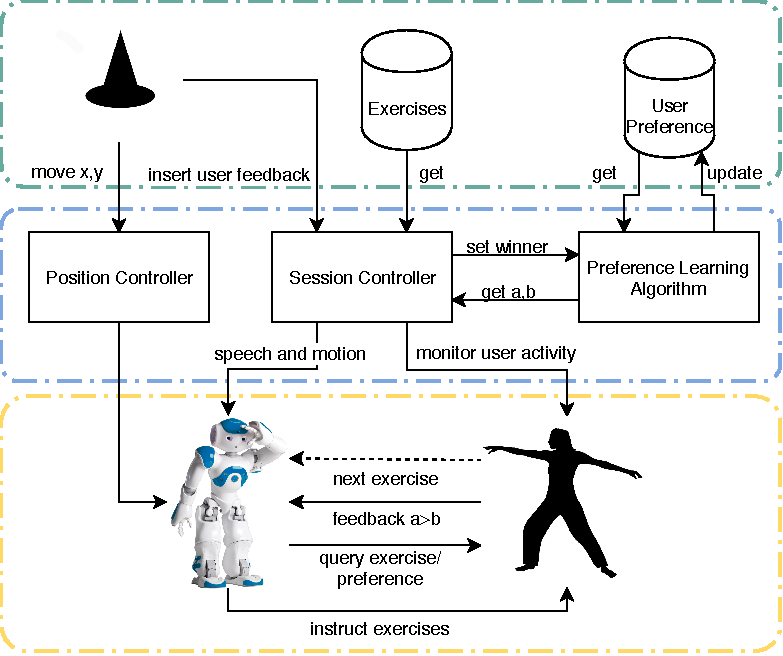
\includegraphics[width=\columnwidth]{figures/figure-latex/systeminteraction.pdf}
\caption{System and interaction overview for the \textit{adaptive} robot condition.} \label{fig:system}
\end{figure}

\hypertarget{ecercise-database}{%
\subsection{Exercise Database}\label{ecercise-database}}

As previously found, exercising preference is individual for each person
\autocite{rhodes2006personality}. Thus, for the aim of this study, we
developed a system that provides a variety of different exercises. We
have chosen 25 exercises in total from 5 different categories: strength,
stretch, cardio, Taichi, and meditation. This set of exercises tackles
one of the open issues in \glspl{sar} for exercising tasks. Previous work often
looked at a single type of exercises like arm movements
\autocite{eriksson2005hands,fasola2013socially,guneysu2017}. The
approach of using a spectrum of different exercises might show that
people can perform various exercises together with a robot.

Table \ref{tab:pl:exercises} presents the list of the chosen exercises. They
have been selected based on a variety of criteria: a) the possibility to
animate and execute them on Nao (\ie{}, Nao cannot jump.), b) the
difficulty that users can perform them (\ie{}, exercises should not be
too challenging for the participants), c) the exercises should challenge
the full embodiment of the robot (\ie{}, laying down, balancing,
standing).

Moreover, we limited the set of exercise to five categories and five exercises per category due to two considerations. 
First, we chose five categories to make sure that the user is presented at least once every combination of exercising categories, which will be important for the preference learning approach that relies on the comparison between exercising categories\footnote{Using five exercising categorires results in  ${5}\choose{2}$ = 10 possibble comparisons. Adding another category would result in ${6}\choose{2}$ = 15 possible comparisons, which would increase the total experiment time.}. Second, we chose five exercises per category so that the user's eventually try out some other categories after the exercises start repeating. 

All of them have been animated on Nao using Choregraphe
\autocite{pot2009choregraphe,gouaillier2008nao}. Figure
\ref{fig:exercises} shows an example of a user exercising together with
the robot.

\begin{center}
\begin{table*} [t!]
\centering
\captionsetup{justification=centering}
\caption{Used exercises for the presented study.}\label{tab:pl:exercises}
\begin{tabular}{@{} *5l @{}}    \toprule
% \emph{name} & \emph{foo} &&&&  \\\midrule
Strength  & Stretch & Cardio & Meditation & Taiji Drills \\ \midrule
  Push up & Neck    & Jumping Jacks & The boat & Golden rooster \\
Squats & Triceps & Front Lunge & 9 breathes & Rainbow\\
 Crunches & Hip  & Side Lunge & relaxation & Punch\\
 Superman & Quadriceps & Boxing & Inner light & Parting kick\\
 Bridge & Side  & Mnt. Climbers & Piece sign & Lifting water\\\bottomrule
% \bottomrule
\end{tabular}
\end{table*}
\end{center}

\begin{figure}[h!]
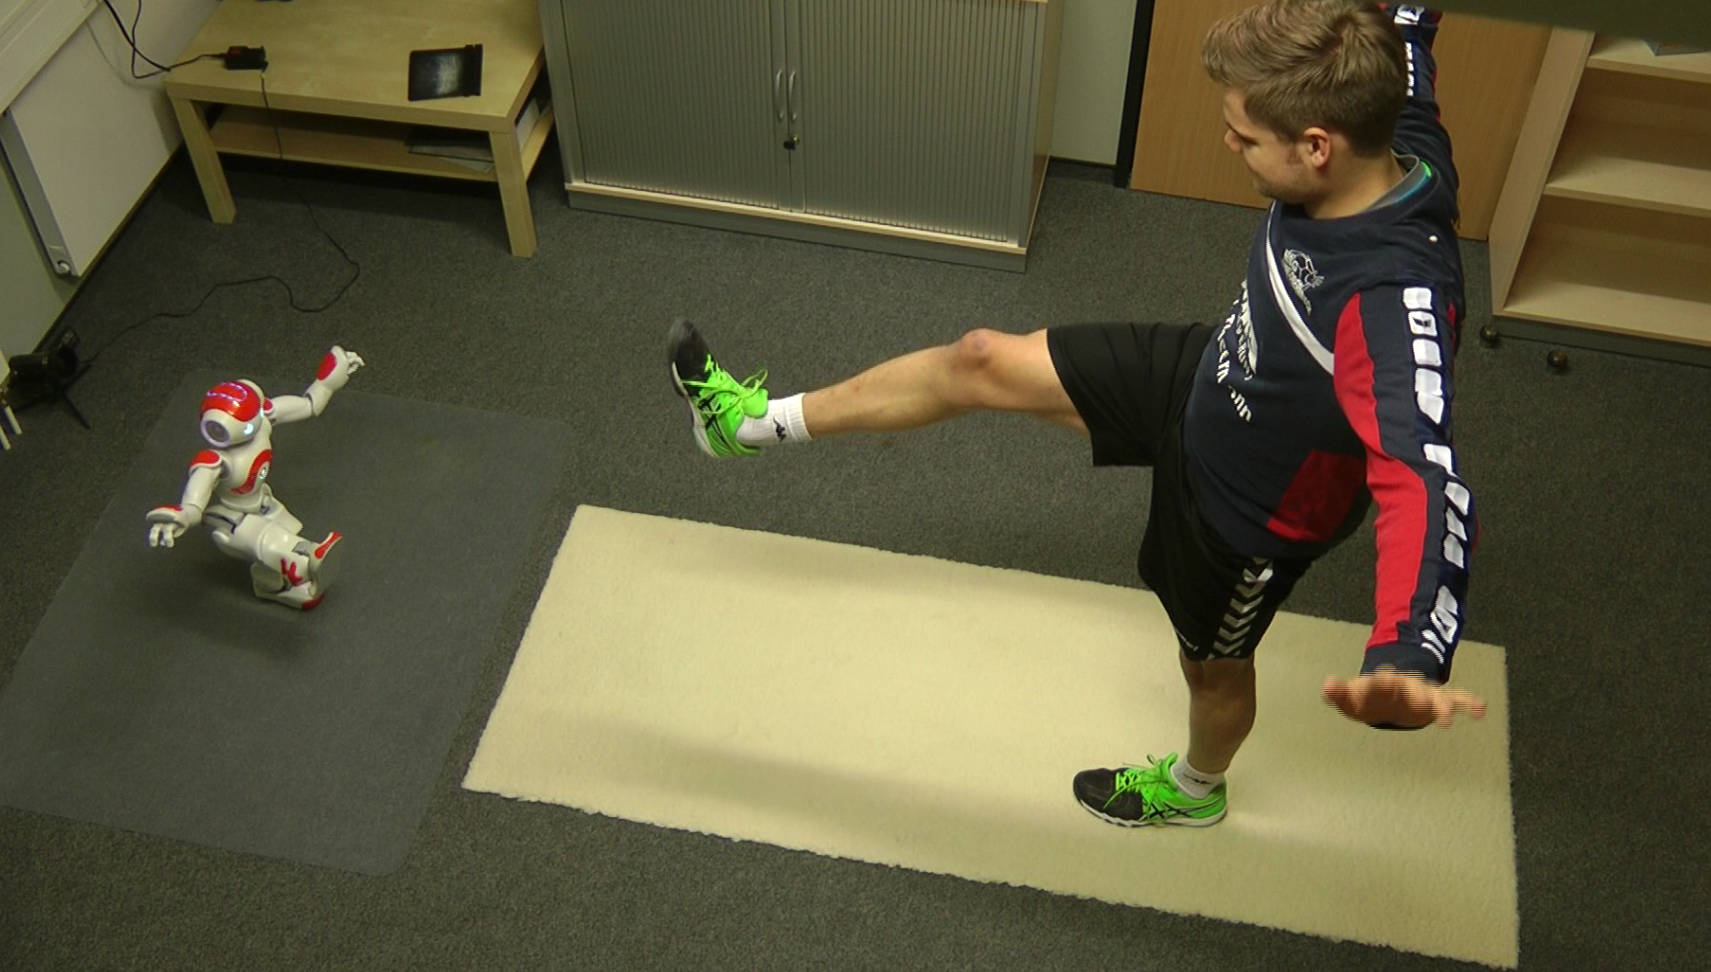
\includegraphics[width=\columnwidth]{figures/taichi.png}
\caption{Robot and user performing the Taiji drill \textit{Parting kick} together.} \label{fig:exercises}
\end{figure}

\hypertarget{preference-learning-framework}{%
\subsection{\texorpdfstring{Preference Learning Framework
\label{sec:framework}}{Preference Learning Framework }}\label{preference-learning-framework}}

% % This section will briefly introduce preference learning as a formal
% problem from the perspective of the Multi-Armed Bandit problem.

Preference learning is a subfield of machine learning that aims to learn
predictive models from previously observed information (\ie{},
preference information) \autocite{Fuernkranz2011}. In supervised
learning, a data set of labeled items with preference information is
used to predict preferences for new items or all the other items from a
data set. In general, the task for preference learning is concerned with
the problem of learning to rank.

There are many different approaches to preference learning. It can be
solved using supervised learning, unsupervised learning and also
reinforcement learning. Since there exists no particular data set we
could use for supervised or unsupervised learning, it is challenging to
build a model that can predict preferences from previously observed
information. Therefore, we are focusing on how the system can learn an
initial preference relation for a given itemset without any prior
information (\ie{}, the cold start problem). Thus, we are trying to
solve the preference learning problem using online methods for the
Multi-Armed Bandit problem or more precisely Dueling Bandit algorithms
\autocite{yue2012k}.

The dueling bandit problem consists of \(K\)(\(K\geq2\)) arms, where at
each time step \(t>0\) a pair of arms
(\(\alpha_{t}^{(1)},\alpha_{t}^{(2)}\)) is drawn and presented to a
user. A noisy comparison result \(w_{t}\) is obtained, where \(w_{t}=1\)
if a user prefers \(\alpha_{t}^{(1)}\) to \(\alpha_{t}^{(2)}\), and
\(w_{t}=2\) otherwise. The distribution of the outcomes is presented by
a preference matrix \(P=[p_{ij}]_{KxK}\), where \(p_{ij}\) is the
probability that a user prefers arm \(i\) over arm \(j\)
(\eg{},\(p_{ij} = P\{i\succ j\}, i,j = 1,2,..,K).\)).

The goal of the preference learning task is, given a set of different
actions (\eg{}, different sport categories), to find the user's
preference order for these categories by providing the user two
\(\alpha_{i}\) and \(\alpha_{j}\) and update the user preferences based
on the selection of the preference between \(\alpha_i\) \(\succ\)
\(\alpha_j\) or \(\alpha_i\) \(\prec\) \(\alpha_j\).

Thus, the challenge is to find the user's preference by running an
algorithm that balances the exploration (gaining new information) and
the exploitation (utilizing the obtained information). In this work, we
are using the \gls{dts} algorithm presented in
\autocite{wu2016double}. Since there are several implementations to
solve the dueling bandit problem we need to answer the question of why
we have chosen this specific kind of algorithm.

Two reasons mainly drive this decision, the state of the art algorithms
at the time of this study were \gls{dts}, RMED and its successor ECW-RMED
\autocite{komiyama2015regret,komiyama2016copeland}. Both perform
reasonably well regarding their asymptotic behavior. However, at this
point, we are not interested in the long-term run of these algorithms
but in the initial phase. If one takes a look at the first steps of
these algorithms, one can see a significant difference between them that
likely influence the \gls{hri} experience. RMED and ECW-RMED both have an
initial phase where all possible pairs are repeatedly drawn for some
time (see Algorithm 1 \autocites{komiyama2015regret}{komiyama2016copeland}).
From an algorithmic perspective this is reasonable, but looking at it
from the viewpoint of the interaction, this would lead to systematic
comparisons that could result in boredom and even annoyance when the
interaction partner is seemingly interrogating the user for her/his
preferences. Thus, we assume that the \gls{dts} algorithm is more useful for
\gls{hri}(especially for the initial contact between the trainee and the
robot coach), because it does not rely on a systematic comparison of all
possible pairs.

\hypertarget{session-manager-system-and-interaction-flow}{%
\subsection{Session Manager: System and Interaction
Flow}\label{session-manager-system-and-interaction-flow}}
The system waits for a user to be present in the room. Depending on the
distance, it asks the participant to come closer. The system introduces
itself to the user, explains its behavior and asks whether the user
wants to start the exercising program. Afterward, in the \textit{adaptive}
condition, the algorithm selects two exercises from the database, and
Nao instructs the user to do the exercises. Following, it asks the
participant which kind of exercises she or he prefers (preference
feedback).

At the beginning, we used the internal speech recognition of Nao.
However, prototype experiments showed that the speech recognition
capabilities are below an acceptable recognition rate, therefore we
manually inserted the user's feedback using a~\gls{woz} style.
Additionally, when Nao performs the exercises, it moves away from the
initial position. We have implemented a simple marker based localization
strategy. However, the duration for localization and position creates an unsatisfying interaction experience. Since this long time is a significant disturbance for
the \gls{hri}experience, we also have implemented a~\gls{woz} position controller
to move the robot to the correct position manually after each exercise.

The primary interaction flow for the \textit{adaptive} conditions continues as follows:
Based on the current user's preference database the algorithm selects
two exercises, then the session manager runs these exercises
sequentially. During the exercises, the session manager receives user
skeleton information and monitors whether the user is doing the
exercises. This exercising information was used to synchronize the
exercising speed of the user and the robot. Afterward, the robot asks
the user which of the exercises she or he prefers. The wizard listens to
the user's feedback using an installed microphone in the experimental
room and feeds the user's input back to the session manager. The robot
acknowledges the decision by repeating the chosen exercise. The
preference learning algorithm updates the user's preference database and
selects the next exercises based on the current user preference.

\hypertarget{sudy-design}{%
\section{\texorpdfstring{Sudy Design
\label{adaptation:sec:study}}{Sudy Design }}\label{sudy-design}}

We conducted a study with a between-subject design (\textit{adaptive} robot
vs.~\textit{adaptable} robot) where participants were randomly assigned to one of
two conditions.

\hypertarget{conditions}{%
\subsection{Conditions}\label{conditions}}

\hypertarget{adaptivity}{%
\paragraph{adaptive}\label{adaptivity}}

The robot in the adaptivity condition used the algorithm described in
\autocite{wu2016double}. During the introduction phase, the system
explains to the user that it will do different exercises together with
the user and will ask for preference feedback relating to the different
exercises. At each time step, the system selects two exercises based on the preference learning algorithm and
executed them consecutively with the user. Afterward, the system queries
the user for a preference statement. This behavior repeats for 14
exercises (or seven comparison iterations). After the 14 exercises, the system asks
whether the user wants to continue exercising for two more exercises or
quit the experiment. After the two additional exercises, the robot
finishes the interaction. It states the user's learned preferences and
thanks for the participation. We limited the additional exercises to two
exercises, due to battery concerns and overheating of joints.

\hypertarget{adaptability}{%
\paragraph{adaptable}\label{adaptability}}

The robot in the adaptability condition did not use any preference
learning algorithm and did not select the next exercises autonomously.
In the introduction phase, the system explains that it offers different
exercises they can do together. The robot verbally listed the possible
exercising categories in a randomized order and the user could choose
the exercise category she or he wants to experience. Thus, the user was
in control of the exercise session and could choose the exercise
category she or he prefers. Also in this condition, the human and robot
did 14 exercises together, and the robot asked whether the user wants to
do two additional exercises.

\hypertarget{participants}{%
\subsection{Participants}\label{participants}}
Due to the expensiveness of this experiment in terms of time costs (\ie{}, 2 hours per subject), we limited our sampling to 20 subjects per group. However, due to prior testing and experiments, we are expecting a large effect size for our hypothesis relevant measurements. The power analysis with a significance level of $\alpha$ = .05 and n=20 per cohort revealed a 70\% power. Though, we know that power analysis may not be accurate and that our estimate could prove wrong, we expect that this sample size will be sufficient for determining a statistical effect with a large effect size and sufficient power. 
The sampled participants (\(N\) = 40; average age \(M\) = 26.02, \(SD\) = 5.48, 13
female and 7 male in the adaptivity condition; 12 female and 8 male in
the adaptability condition) were mostly university students that were
acquired by information on the campus and social media. The majority of
the participants were naive robot user and had no background in computer
engineering or programming.

\hypertarget{procedure}{%
\subsection{Procedure}\label{procedure}}

Participants arrived at the lab individually. First, they had to sign a
consent form. Then, the experimenter led the participants to a room
where they can change their clothes. Later, they were told to enter the
lab and follow the instructions of the system. Until this point, the
participants did not know that they will be interacting with a robotic
system. We neglected this prior information to not bias the participants
or raise false beliefs. Then the participants entered the lab without
the experimenter. The interaction took approximately 50 to 60 minutes,
and the experimenter monitored the experiment from a control room. After
the interaction finished, participants had to answer a questionnaire and
had a voluntary post-study interview. Finally, they were debriefed and received 8 Euros
for their participation. The ethical committee of our university
approved the procedure.

\hypertarget{measurements}{%
\subsection{Measurements}\label{measurements}}

In this study, we are investigating whether different personalization
methods change a user's subjective perception of the robot, the alliance
to it and motivation to interact with the system. The following measures
were used in this study to find evidence for our presented hypotheses.
We used Cronbach's \(\alpha\) as a measure for the internal consistency
of the scales \autocite{cronbach1951coefficient}.

\hypertarget{negative-attitudes-towards-robots}{%
\paragraph{Negative Attitudes Towards
Robots}\label{negative-attitudes-towards-robots}}

Attitudes towards robots were measured using the \gls{nars}, \(\alpha\) = .8, on a five-point
Likert scale \autocite{nomura2006experimental}. Negative attitudes
towards robots could be a confounding factor explaining results obtained
on the perception of the robot.

\hypertarget{physical-activity-enjoyment}{%
\paragraph{Physical Activity
Enjoyment}\label{physical-activity-enjoyment}}

Participants rated their physical training enjoyment using the \gls{paes}, \(\alpha\) = .91
\autocite{kendzierski1991physical}. The average overall item responses
calculate the overall enjoyment score.

\hypertarget{system-usability}{%
\paragraph{System Usability}\label{system-usability}}

System's usability was measured by the \gls{sus}
,\(\alpha\) = .84, with ten items on a 5-point Likert
\autocite{brooke1996sus}.

\hypertarget{team-perception}{%
\paragraph{Team Perception}\label{team-perception}}

We measured the user's perceived team perception using scales from
\autocite{nass1996can}. These scales measure the general team perception
(\(\alpha\) = .38), the openness to suggestions from the team member
(\(\alpha\) = .94) and the perceived cooperation (\(\alpha\) = .39).
All scales were on a 5 point-based Likert-scale.

\hypertarget{perception-of-the-partner}{%
\paragraph{Perception of the
Partner}\label{perception-of-the-partner}}

Participants were asked to rate the perception of the robot on the
\gls{rosas}. This scale includes the
perceived warmth (\(\alpha\) = .85), competence (\(\alpha\) = .77) and
discomfort (\(\alpha\) = .76) on a 9 point-based Likert-scale
\autocite{carpinella2017robotic}.

\hypertarget{motivation}{%
\paragraph{Motivation}\label{motivation}}

To have an additional measure to see whether people are interested in
exercising a second time with the robot, we let the participants opt-in
for voluntarily exercising with the robot again without monetary
compensation. Participants were asked at the end of the questionnaire to
enter their email address if they want to exercise again in the
following week.

\hypertarget{alliance-and-trust-1}{%
\paragraph{Trust in Alliance}\label{alliance-and-trust-1}}

Finally, we used the \gls{wai}, \(\alpha\) = .91,
as a measure commonly used in helping alliances to assess trust and
belief in a common goal of helping that a therapist, clinician or coach
has for another \autocite{horvath1989development}. This measure has
recently been used in \gls{hci} and \gls{hri} studies for assessing the alliance
and trust between the human and a \gls{sar}.
\autocite{bickmore2005establishing,kidd2008robots}.

\hypertarget{results}{%
\section{\texorpdfstring{Results
\label{adaptation:sec:results}}{Results }}\label{results}}
In this section, we present the results from our quantitive survey evaluation, from post-study interviews and preference learning results.

Data were analyzed using the statistical computing language R
\autocite{R2013}. We analysed the data for normality assumptions and used
Welch's two-sample t-test if the data meet the criteria and Wilcoxon
rank sum test respectively
\autocite{welch1947generalization,wilcoxon1945individual}. To increase
reproducible science, we published the
data and scripts for the analysis on Github\footnote{\url{https://github.com/sebschne/ijsr2019}}.

\begin{figure*}[bt!]
\centering
\includesvg[width=2.\columnwidth]{figures/figure-latex/neo-ffi} \caption{\label{fig:adapt:neoffi} Boxplot showing the user ratings for the NEO-FFI personalty test.}\label{fig:unnamed-chunk-4}
\end{figure*}
\subsection{Quantitative Results}
\hypertarget{manipulation-check}{%
\paragraph{Manipulation Check}\label{manipulation-check}}

The data was checked for differences in the participant's previous
experience with technology, their average weekly exercising activity, personality, physical activity enjoyment (PAES) and
the attitudes towards robots. Previous experience (\(W\) = 146.5, \(p\)
= .15), exercising activity (\(W\) = 237, \(p\) = .45), \gls{paes} (\(W\) = 164, \(p\) = .34, \(r\) = -.96), as well as \gls{nars}
(\(t(37.7)\) = 1.78, \(p\) = .08) were not significantly different between the conditions. Thus, the manipulation seems to be succesful. 

\begin{figure}[bt!]
\includesvg[width=\columnwidth]{figures/figure-latex/sus} \caption{\label{fig:adapt:paes} Boxplot showing the user ratings for perceived cooperation, system usability, physical activity enjoyment, and working alliance.}\label{fig:unnamed-chunk-4}
\end{figure}

% \hypertarget{cooperation}{%
% \subsection{Cooperation}\label{cooperation}}
% 
% The results for the cooperation scale are depicted in
% \autoref{fig:adapt:paes}. A Welch's two-sample t-test showed a
% significant difference between the conditions for cooperation,
% \(t\)(37.91) = -2.43, \(p\) = .02, \(d\) = .77 The \textit{adaptive} system has
% been rated as significantly more cooperative (\(M\) = 3.7, \(SD\) = .66)
% than the \textit{adaptable} system (\(M\) = 3.2, \(SD\) = .63). However, this
% result can only be carefully considered due to the low internal
% consistency of the cooperation scale (\(\alpha\) \textless{} .4).
% The results for the RoSAS are plotted in \autoref{fig:adapt:rosas} and the results for the .
The general hypothesis unrelated measurements show that participants did not evaluate the usability of the systems significantly different, \(t\)(35.56) = .95, \(p\) = .35, \(d\) = .30. There was also no significant different evaluation regarding the openness to follow the system's suggestions, \(W\) = 204, \(p\) = .92, \(r\) = -.10 (see Figure~\ref{fig:adapt:paes}). Also, participants did not feel significantly more discomfort between the conditions, (\(W\) = 210, \(p\) = .80, \(r\) = -.26 (see Figure \ref{fig:adapt:rosas}).

However, the systems was perceived as more warmth on subscale of the \gls{rosas} scale, \(t\)(36.23) = -2.47, \(p\) = .02, \(d\) = .78. The \textit{adaptive} system is perceived as warmer (\(M\) = 4.08, \(SD\) = 1.62) than the \textit{adaptable} system (\(M\) = 2.93, \(SD\) = 1.29).


% \hypertarget{system-usability-1}{%
% \subsection{System usability}\label{system-usability-1}}
% 
% A Welch's two-sample t-test for differences on the SUS scale showed no
% significant differences, \(t\)(35.56) = 0.95, \(p\) = .35, \(d\) = .30.

% \hypertarget{openness}{%
% \subsection{Openness}\label{openness}}
% 
% A Wilcoxon rank sum test with continuity correction showed no
% significant differences between the two conditions on the openness to
% influence scale, \(W\) = 204, \(p\) = .92, \(r\) = -.10

% \hypertarget{physical-activity-enjoyment-1}{%
% \subsection{Physical Activity
% Enjoyment}\label{physical-activity-enjoyment-1}}
% 
% A Wilcoxon rank sum test with continuity correction showed no
% significant difference between the two condition on the PAES scale,
% \(W\) = 164, \(p\) = .34, \(r\) = -.96.

% \hypertarget{perception-of-the-partner-1}{%
% \subsection{Perception of the
% Partner}\label{perception-of-the-partner-1}}
% 
% The results for RoSAS are plotted in \autoref{fig:adapt:rosas}. The
% detailed analysis is listed in the following.

\begin{figure}[bt]
\includesvg[width=\columnwidth]{figures/figure-latex/rosas} \caption{\label{fig:adapt:rosas}Boxplot showing the user ratings for the \gls{rosas}.}\label{fig:unnamed-chunk-6}
\end{figure}

% \hypertarget{warmth}{%
% \paragraph{warmth}\label{warmth}}
% 
% A Welch's two-sample t-test showed a significant effect regarding the
% warmth subscale of the RoSAS scale, \(t\)(36.23) = -2.47, \(p\) = .02,
% \(d\) = .78. The \textit{adaptive} system is perceived as warmer (\(M\) = 4.08,
% \(SD\) = 1.62) than the \textit{adaptable} system (\(M\) = 2.93, \(SD\) = 1.29).

\hypertarget{competence}{%
\paragraph{Hypothesis 1}\label{competence}}

We hypothesized that the competence is perceived as higher in the adaptive condition compared to the adaptable condition. A Welch two-sample t-test confirms this hypothesis and shows a significant difference between the conditions,
\(t\)(34.55) = -2.49, \(p\) = .02, \(d\) = .79. The \textit{adaptive} system is indeed
perceived as more competent (\(M\) = 6.55, \(SD\) = 1.67) than the
\textit{adaptable} system (\(M\) = 5.4, \(SD\) = 1.2).
% 
% \hypertarget{discomfort}{%
% \subsubsection{discomfort}\label{discomfort}}
% 
% There were no significant difference between the conditions determined
% by a Wilcox-ranked sum test (\(W\) = 210, \(p\) = .80, \(r\) = -.26) on
% the discomfort scale.


\hypertarget{working-alliance}{%
\paragraph{Hypothesis 2}\label{working-alliance}}
We also hypothesized that the user's trust in the \gls{hra} is higher in the adaptive condition. The results of the \gls{wai} are depicted in \autoref{fig:adapt:paes}. A Welch
two-sample t-test revealed significant difference between the
conditions, \(t\)(36.05) = -3.17, \(p\) = .003, \(d\) = 1.00. The
\textit{adaptive} system has been rated significantly higher on the alliance
inventory (\(M\) = 2.8, \(SD\) = .93) than the \textit{adaptable} system (\(M\) =
1.99, \(SD\) = .76). This confirms our hypothesis H2.

\begin{figure}[bt!]
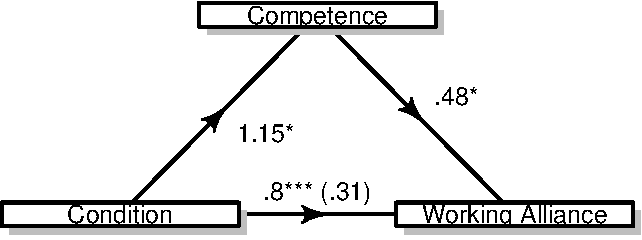
\includegraphics[width=\columnwidth]{figures/figure-latex/unnamed-chunk-9-1} \caption{\label{fig:adapt:mediation}Standardized regression coefficients for the alliance between conditions and user's alliance with the robot as mediated by the user's perceived competence of the robot. The standardized regression coefficient between the conditions and the WAI, controlling for perceived competence, is in parentheses.}\label{fig:unnamed-chunk-9}
\end{figure}
\paragraph{Hypothesis 3}
To assess whether the condition's effect on overall alliance was
statistically mediated by perceived competence, we used non-parametric
bootstrapping method based on the method from
\autocite{preacher2008asymptotic} and coded condition as adaptable =
0, adaptive = 1. We tested assumptions for a mediation analyis using
the \texttt{gvlma} package and used the \texttt{mediation} package to do
the analysis. This analysis confirmed that perceived competence
statistically mediated the alliance between \textit{adaptive} condition and
overall trust in the robot (ACME = .48, \(p\) \textless{} .05, 95\% CI =
.1 to .91; 10,000 resamples; see \autoref{fig:adapt:mediation}) with no
direct effect of autonomy of the system (ADE = .31, \(p\) = .09) and
significant total effect (\(p\) \textless{} .001).


\hypertarget{motivation-to-interaction}{%
\paragraph{Hypothesis 4}\label{motivation-to-interaction}}
Hypothesis 4 states that participants in the adaptive condition would voluntarily exercise a second time with the system compared to the adaptable system. 
The ratio for participant's wish to voluntarily repeat the interaction
is depicted in \autoref{tab:pl:mot}. Pearson's Chi-squared test
showed that participants opted more often to exercise again with the
\textit{adaptive} condition (\(\chi\) = 4.80 , \(d.f.\) = 1, \(p\) = .03). This
effect is however not persistent when using Yates' continuity correction
(\(\chi\) = 3.33, \(d.f.\) = 1, \(p\) = .07). Thus, our Hypothesis 4 is just partially supported.

\begin{center}
\begin{table} [ht!]
\centering
\captionsetup{justification=centering}
\caption{Paricipants count to voluntarily repeat the interaction.}\label{tab:pl:mot}
\begin{tabular}{@{} *3l @{}}    \toprule
% \emph{name} & \emph{foo} &&&&  \\\midrule
  & yes &  no \\ \midrule
  adaptive & 18    & 2 \\
 adaptable & 1  & 19 \\\bottomrule
% \bottomrule
\end{tabular}
\end{table}
\end{center}


\subsection{Preference Learning Results}

The results for the learned exercising preferences by the system are depicted in Figure \ref{fig:userranking}. The plot shows for each participant in the \textit{adaptive} condition the user's own \textit{ranked} preference set and the \textit{learned} exercising preference from the system. Figure \ref{fig:distances} shows the measured differences between the learned rankings and true rankings in a box plot. We highlight three different measurements that are used to compare item rankings.  The position distance shows that the difference between the ranked position of the user's most prefered item in relation to the position where the learner has ranked it. The median for this ranking is 0, presenting evidence that for most users the system was able to identifiy the users most preferred exercise after a very short interaction time. This is a promising result, presenting evidence that these kind of learning algorithms indeed seem suitable to decrease the gap between user's preference and the system's behavior. It is important to notice here, that the system was not able to correctly rank the most preferred item. However, it never ranked the user's most preferred item on the last position. The only extreme example where the preference learning did not work out at al was for participant PB2 and PB13.  

\begin{figure*}
\includesvg[width=2.\columnwidth]{figures/figure-latex/user_rankings} \caption{\label{fig:adapt:mot}Individually ranked and learned exercising preference for the different exercising categories .}\label{fig:userranking}
\end{figure*}

\begin{figure}
\includesvg[width=\columnwidth]{figures/figure-latex/distances} \caption{\label{fig:adapt:mot}Hamming, position and discounted distances between the learned and user ranked exercising preferences.}\label{fig:distances}
\end{figure}
'
% https://app.mindmup.com/map/_free/2019/05/7ec8f8907bc311e99ec4af2da182d04c


\subsection{Qualitative Results}

To better understand how participants felt motivated by the robot and used the personalization mechanism, we conducted semi-structured post-study interviews. After participants finished the questionnaire, we asked them whether they would like to also answer some interview questions. Most of the participants gave, at least, some short responses. We asked the participants
\begin{enumerate}
 \item whether and why they felt motivated by the system 
 \item we asked participants which strategy they used to select the exercises in the \textit{adaptable} condition
 \item in the \textit{adaptive} condition, we asked participants on which criteria they made their preference selection.
 \item how much money they would spend for such a system.
\end{enumerate}
The following paragraphs briefly sketch the interview responses.

% \paragraph{First impression}

\paragraph{Exercising Motivation}
Six participants in the \textit{adaptable} condition said that the system motivates them to exercise (e.g.,~\textit{PA14}: Motivating, very nice during static workouts but not so good for cardio). In contrast, five participants stated that the system was not motivating or that they are intrinsically motivated and would not need it, but they would appreciate assistance when they are injured (e.g.,\textit{PA12}:`` I don't know. I am intrinsically motivated. For my daily live I would not use it, perhaps if I am injured as a rehabilitation tool.``)

Eleven participants in the \textit{adaptive} condition stated that the system would motivate them, while five said that they did not feel motivated by it. 
Table \ref{tab:pl:testimonies} presents some testimonies of the participants. Participants responded in various ways, reflecting their internal heuristic to evaluate whether and why they felt motivated. The responses show that there are great differences in the evaluation criteria for each person. Participants felt either motivated by the appearance of the robot, the novelty of guiding them through new exercises, the fact that they do not feel evaluated by a robotic exercising partner, the companionship the robot can provide, as well as the possibility that the robot can quantify their training progress. Participants who stated that they did not feel motivated by the systems gave recommendations and use case suggestions for the system. The suggested use case for the system would be as a reminder system, as a partner for rehabilitative exercises or as a partner for people that just started exercising. As interactive suggestions, participants proposed that the robot should be faster and emulate emotions.   

\begin{center}
\begin{table*} [t!]
\centering
\captionsetup{justification=centering}
\caption{User response (\textit{adaptive} condition) on the question whether and why they felt motivated by the system.}\label{tab:pl:testimonies}
\begin{tabular}{lll}    \toprule
% \emph{name} & \emph{foo} &&&&  \\\midrule
ID  & Response & Reason \\ \midrule
  PB6 & \parbox[t]{1.4\columnwidth}{''I would motivate a lot of people. For me, I would have to \textbf{decide} on my own which exercises we're doing.''}
 & self-determination \\
%   
  PB7 & ''It motivated me to \textbf{try out} new things.'' & novelty  \\
%   
PB9 & ``The robot was \textbf{sweet}, it was enjoyable'' & appearance \\
% 
 PB10 & \parbox[t]{1.4\columnwidth}{``It's nice when \textbf{somebody is around} who shows you the exercises and gives you structure. Especially, when you don't have much time''} & companionship \\
%  
 PB12 & \parbox[t]{1.4\columnwidth}{``It would motivate me when it is better developed. Currently, I just exercise with videos, it could replace exercising vides when it is more sophisticated. I would prefer it to a human  partner or coach. The robot keeps a distance and \textbf{does not judge me}, it could feel more uncomfortable with a human partner''}  & judgement \\
%  
 PB13 & \parbox[t]{1.4\columnwidth}{``the \textbf{appearance} of the robot motivated me to follow its instructions and trust it. If a smartphone would ask me to do some exercises, I would just swipe them away, but a robot motivates me to try out new exercises.''}  & appearance, embodiment\\
%  
 PB16 & ``It was more fun, because I was \textbf{not alone}'' & companionship \\
%  
 PB18 & \parbox[t]{1.4\columnwidth}{`` I would use it, because I think it's cool. It would be a nice feature, if it could \textbf{track} my performance. I had bad experiences with fitness tracking devices, but a robot could be a companion for everything.''}  & quantifying \\
 
 PB19 &\parbox[t]{1.4\columnwidth}{``Yes it helped me, because I am \textbf{not easily intrinsically} motivated''} & extrinsical factor \\
& & \\
 \bottomrule
% \bottomrule
\end{tabular}
\end{table*}
\end{center}

% ich finde es gut wenn jemand uebungen vorgibt und die zeit hat, roboter eher nicht das mittel meiner wahl, lieber videos weil bewegung geschmeidig sind und die uebungen nicht passen, fuer jemanden der wenig mit sport zu tun hat koennte es schwierig werden wenn man es falsch macht
% motiverter aber nicht mit roboter, weil der roboter keine anstrengung fuehlt, vor machen vl. Fuer rehauebungen
% eher weniger die uebungen waren zu langsam, fuer anfaenger als fuer leute die sport machen
% viele menschen wueder es motivieren, ich muesstes selbst entscheiden was wir machen
% fehlt emotion, mehr motivierend sein. Habe die aussagen nicht ernst genommen wusste das es nur eine maschine ist, ist kein mensch, ich wusste nicht ob er es wahr nimmt
% wenig mit sport zu tun hat koennte es schwierig werden wenn man es falsch macht
% brauche keine externe motivation, fuer vorschlaege offen, habe einfach so gemacht
% sehr starke eigene motivation, glaube nicht dass mich der roboter in den arch trete, generl keine motivation es anzumachen, koennte mich aufregen, eine gue erinnerung was zu machen fuer zu hause eher nicht


\paragraph{Exercise Selection Strategy}
We asked the participants in both conditions, whether they used any strategy to select the next exercise and on which basis they chose their exercising preferences.

In the \textit{adaptable} condition, 10 participants said that they tried to select everything once to see what the system has to offer (\textit{PA8}: "No strategy, I tried to select everything once"). Seven participants selected the exercises based on their actual exercising preferences (\textit{PA14}: "I selected everything based on my preference. Therefore, I did not select cardio or relaxation exercises").

In the \textit{adaptive} condition, ten participants selected the exercises based on their current enjoyment of the task (e.g.,~\textit{PB9}: I thought about what was more fun for me and picked the exercise accordingly), and three selected the activities based on their actual exercising preference (e.g.,\textit{PB18}: I chose the exercises based on my choice).

It is interesting to note that the interview responses show that the different types of personalization strategy lead to different approaches to select the exercises. While in both conditions, there were participants that chose activities based on their actual preference, participants that did not use a favorite based selection approach used mainly two different kinds of selection criteria. Participants in the \textit{adaptable} condition stated more often than they used their curiosity as selection criteria (e.g., ``I wanted to see what the system has to offer''). In contrast, participants in the \textit{adaptable} condition did not state that they used curiosity criteria. Instead, they used enjoyment as the salient criteria for stating their exercising preference.

This presents evidence that people use a different kind of qualitative criteria to maximize their interactive experience. In \textit{adaptable} condition, participants concentrated more on the novelty as an evaluation criterion while in the other condition, participants used their enjoyment as an evaluation criterion. Though maximizing novelty can also be considered as an interaction enjoyment criterion, it is sufficiently different from the actual enjoyment evaluation. Maximizing novelty tries to optimize expected interaction experience in the future, while the other approach only evaluates the current interaction experience.

\paragraph{Costs}
We asked participants how much they would pay for such a system. Their responses were ambigious and we found a big discprepancy on how much they are willing to pay for such a system and how much they think it would actually cost. While many knew that robots are expensive, the willingness to pay this amount is actually low. Thus, we concentrate only on the expenses they are willing to pay. The median amount of money participants in the adaptive condition would pay is 250\euro, while in the adaptable condition, participants would pay 300\euro. Eventhough, the median is higher for the adaptable condition, the variance is greater for the adaptive condition. Since the resutls are not significantly different ($t$(24.53) = .3, $p$ = .72), we assume that the personalization strategy is, not yet, the salient feature to determine the value of the system. Participants rather stated that, if the system is more capable in doing the exercises they would be willing to pay more for it.

\begin{figure}
\includesvg[width=\columnwidth]{figures/figure-latex/costs} \caption{\label{fig:adapt:cost} Box plots showing amount of money participants are willing to pay for the system.}
\end{figure}

\section{Discussion}\label{discussion}
This work investigated how a system's type of personalization mechanism
based on different \gls{loa} alters the user's perception of it. It presented
a study to investigate the effects of interacting with an \textit{adaptable} or
\textit{adaptive} robot on the perceived alliance with the system and
the perceived competence of it depending on different personalization
strategies. Thus, it closes a gap in the research literature on the
effects of different personalization methods in\gls{hri}. The robot in our
study was either indirectly controlled by a user's preference feedback
or directly controlled by the user. In the case of the \textit{adaptive}
condition, we used a preference-learning method based on dueling bandits.
Thus, this work also presents a evidence that these
kinds of algorithms are suitable for personalizing~\gls{hri} experience. The results from our evaluation shows, that the system is, in most of the times, able to learn a user preference during a short exploration phase. 

We hypothesized that different \gls{loa} alters the perceived competence of
the robot and alliance with it. The results present evidence that
users perceive the robot as more competent, which is supported by a
significant difference between the conditions on the \gls{rosas} subscale.
This evidence supports Hypothesis \ref{hyp:adaptability:competence}: An \textit{adaptive}
robot is perceived as more competent than an \textit{adaptable} robot. Further, it confirms theoratically investigations on the \gls{loa} and shows that a system with a higher degree of automation is indeed perceived as more competent. Therefore, we could find a hint that unexpected behaviors result in different evaluations of the robot as postulated in \textcite{epley2007seeing} theory of anthropomorphism. Expectance violations regarding the non-human agent's behavior, let people rethingk their mental model of the agent's behavior or mental state and increases anthropomorphic thoughts. Whether it means that higher degrees of perceived competence also result in higher perceived degrees of anthropomorphism remains uncertain. Though, it is reasonable to argue that also higher competence reflects a higher degree of human-likeness evaluation. Still, it would require further evaluation to discern the effects of competence and anthropomorphism.
% This is also inline with the theory of \textcite{epley2007seeing}, that hypothesises that unexpected behaviors of a system will result in higher 

The results on the perceived alliance with the robot
also supports the Hypothesis \ref{hyp:adaptability:trust}: Participants had a
stronger trust in the alliance with the \textit{adaptive} robot. This result supports the
hypothesis that \textcite{rau2013effects} had, but could not find
evidence to support it. Participants trusted the robot more, if it was
more autonomous than less autonomous. This result seems
counter-intuitive. Why would users trust a robot more, when they
have less control over the robot? It might be that participants also
could have felt overwhelmed by the exercising possibilities they had
with the system. Thus, participants might have felt less burden to
structure the interaction, because the \textit{adaptive} system made the critical
decision. On could say, from a system theory perspective, that the users try to reduce their uncertainty when interacting with the system~\cite{Luhmann2000}. Further, the mediation model supports Hypothesis \ref{hyp:adaptability:mediation} and provides insights on why
the different conditions affected the perceived alliance. Different \gls{loa}
influenced the perceived competence of the system which in turn
increased the alliance to it.
Other researchers showed that anthropomorphism alters the trust in an
autonomous vehicle~\autocite{waytz2014mind}. Higher anthropomorphism
leads to higher confidence in the car. However, these authors have not
measured the perceived competence as an independent mediator. Thus it
remains an open question whether the manipulation of the
anthropomorphism alters the perceived competence in the system and
therefore changes the associated alliance.

% In light of the theory of anthropomorphization, we assumed that an~\textit{adaptive} system could increase the perceived anthropomorphism of the system by showing unexpected behavior~\autocite{epley2007seeing}. We found that users perceive the robot as more competent and warmth. Thus it indicates that the~\textit{adaptive} robot indeed increases the perceived anthropomorphism indirectly measured by the~\gls{rosas}~\autocite{carpinella2017robotic}. However, further studies need to verify this by directly measuring the perceived anthropomorphism.

Finally, we could find partial evidence for Hypothesis~\ref{hyp:adaptability:motivation}. Participants in the~\textit{adaptive} condition opted more often to exercise a second time voluntarily. This result is probably due to the interest in a system that tries to
personalize the interaction by itself. It might raise curiosity and participants are interested to see what other exercises the system can offer or whether the system can effectively learn the user preference. However, this result is only marginally significant after applying a continuity correction. To be sure whether this effect is genuinely
substantial higher sample size is needed.

Our qualitative results also reveal insights in the rational for evaluating different personalization strategies. Using adaptive robots results in evaluation criterias based on the current state, rather than on the already established preference beliefs. This opens speculations wether an adaptive approach leads to reconsider one's beliefs on exercising preference and thus helps to be open for trying new exercises that eventually better fit ones personality. While most participants in the adaptable condition were using their beliefs for the exercising selection, participants in the adaptive condition focussed more on which exercises they enjoed. Having the results for the difference in perceived competence and trust in mind, this shows that participants are open for new suggestions and that they would trust the competence of the system to find the right exercise for them.

One limitation of the interpretation of the results above is the short interaction time during the study. Alliance is build up over repeated interactions between two person. Therefore, the results on the effects of alliance need to be interpreted with caution. Additionally, the scale used in this experiment is primarily designed for measuring the trust and alliance in the client-therapist alliances. Therefore, the results might be different, if we have used a scale that is more focused on the trust in the technical competence of the system. Still, the trust in the relationship is an essential part for long-term \gls{hri} and especially for use cases where the human and robot partner are working towards a long-term goal like increasing physical activity.

Moreover, we have not quantitatively assessed the quality of the preference learning over repeated interactions. Future work will look at the long-term satisfaction regarding the learned preferences. 

\hypertarget{conclusion}{%
\section{\texorpdfstring{Conclusion
\label{adaptation:sec:conclusion}}{Conclusion }}\label{conclusion}}

This work presented a study on different techniques to adjust a \glspl{sar}
behavior towards a user's preference. The results of this study show
that \textit{adaptive} robots are perceived as more competent, warmth and
trustworthy than \textit{adaptable} robots. Thus, the \gls{loa} indeed  has an influence on the interaction experience for the user. Further, it presents evidence that
the perceived competence of the system significantly mediates the
alliance with a system. This mediation effect can be an essential aspect
for long-term interaction with robots and needs in-depth investigations
in long-term studies. The question remains whether an \textit{adaptive} system
can continuously present new and personalized behaviors so that the
system will remain interesting to interact with over time. Moreover, regarding the question how a future social robotic system can personalie it's behavior for the user, our results show that the system is able to sufficiently identifiy the user's preference in a very short amount of time using a \gls{dts} approach. Thus, we could prove, as one of the first researchers to do this, that a qualitative comparative approach is suitable for online adaptation in \gls{hri} scenariso. Nevertheless, the results of this study have to be verfyfied in long-term investigations.

\printglossary

\printbibliography{}

% \bibliographystyle{spbasic}
% \bibliography{mybibfile.bib}

\end{document}
